% Chapter 1

\chapter{Techniques for characterisation} % Main chapter title

\label{Chapter2} % For referencing the chapter elsewhere, use \ref{Chapter1} 

%----------------------------------------------------------------------------------------

% Define some commands to keep the formatting separated from the content 
\newcommand{\keyword}[1]{\textbf{#1}}
\newcommand{\tabhead}[1]{\textbf{#1}}
\newcommand{\code}[1]{\texttt{#1}}
\newcommand{\file}[1]{\texttt{\bfseries#1}}
\newcommand{\option}[1]{\texttt{\itshape#1}}

%----------------------------------------------------------------------------------------

\section{X-ray diffraction Studies}
\begin{figure}[tbh!]
\centering
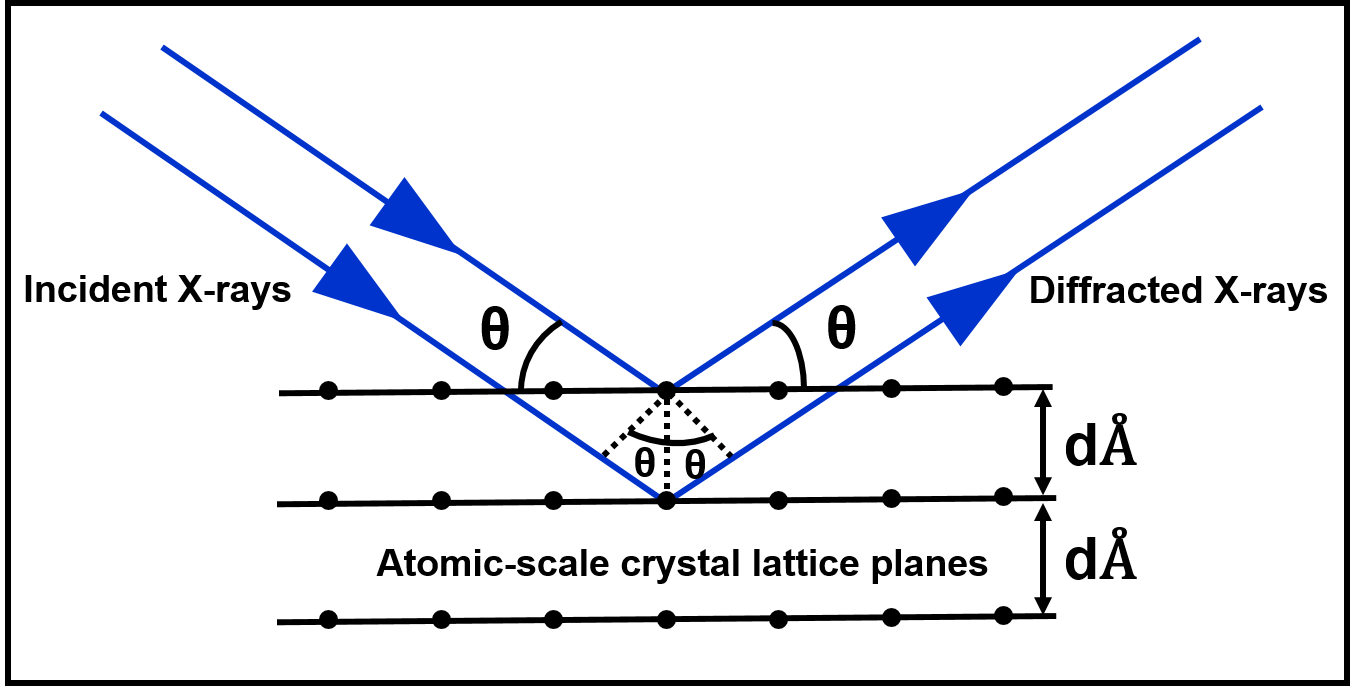
\includegraphics[width=\textwidth]{Figures/XRD}
\caption{Schematic of Bragg's Law}
\label{Figures:XRD}
\end{figure}
X-ray diffraction is the elastic scattering of x-ray photons by atoms in a periodic lattice. The scattered monochromatic x-rays that are in phase give constructive interference. Figure 2.1 illustrates how diffraction of x-rays by crystal planes allows us to derive lattice spacings by using the Bragg's law. As shown in Figure \ref{Figures:XRD}, the electrons present in an atom scatter the X-ray waves. The phenomenon of X-ray striking an electron and releasing secondary spherical waves is called elastic scattering. With the electron as a "scatterer", the array of atoms in a crystal produce spherical waves. The waves add constructively in a few specified directions  and is determined by Bragg's law.
 \begin{equation} \label{eq1}
     2d\sin\theta = n\lambda
 \end{equation}
where d is the spacing between diffracting planes, $\theta$ is the incident angle, n is any integer, and $\lambda$ is the wavelength of the incident beam. We get an X-ray diffraction from an electromagnetic wave striking a repeating arrangement of electrons within the crystal. X-rays produce the diffraction pattern because their wavelength λ is typically the same order of magnitude (1–100 \AA ) as the d-spacing between the crystal planes. According to \ref{eq1} any decrease in 2$\theta$ suggests an increase in the d-spacing. This increase can be attributed to intercalation of ions that take place during electrochemical reactions. XRD helps us detect these changes and determine the cell mechanism.

\section{Raman spectroscopy}

Raman spectroscopy is a technique used to determine vibrational modes of molecules. It is commonly used to provide a structural fingerprint to identify molecules.
\begin{figure}[tbh!]
\centering
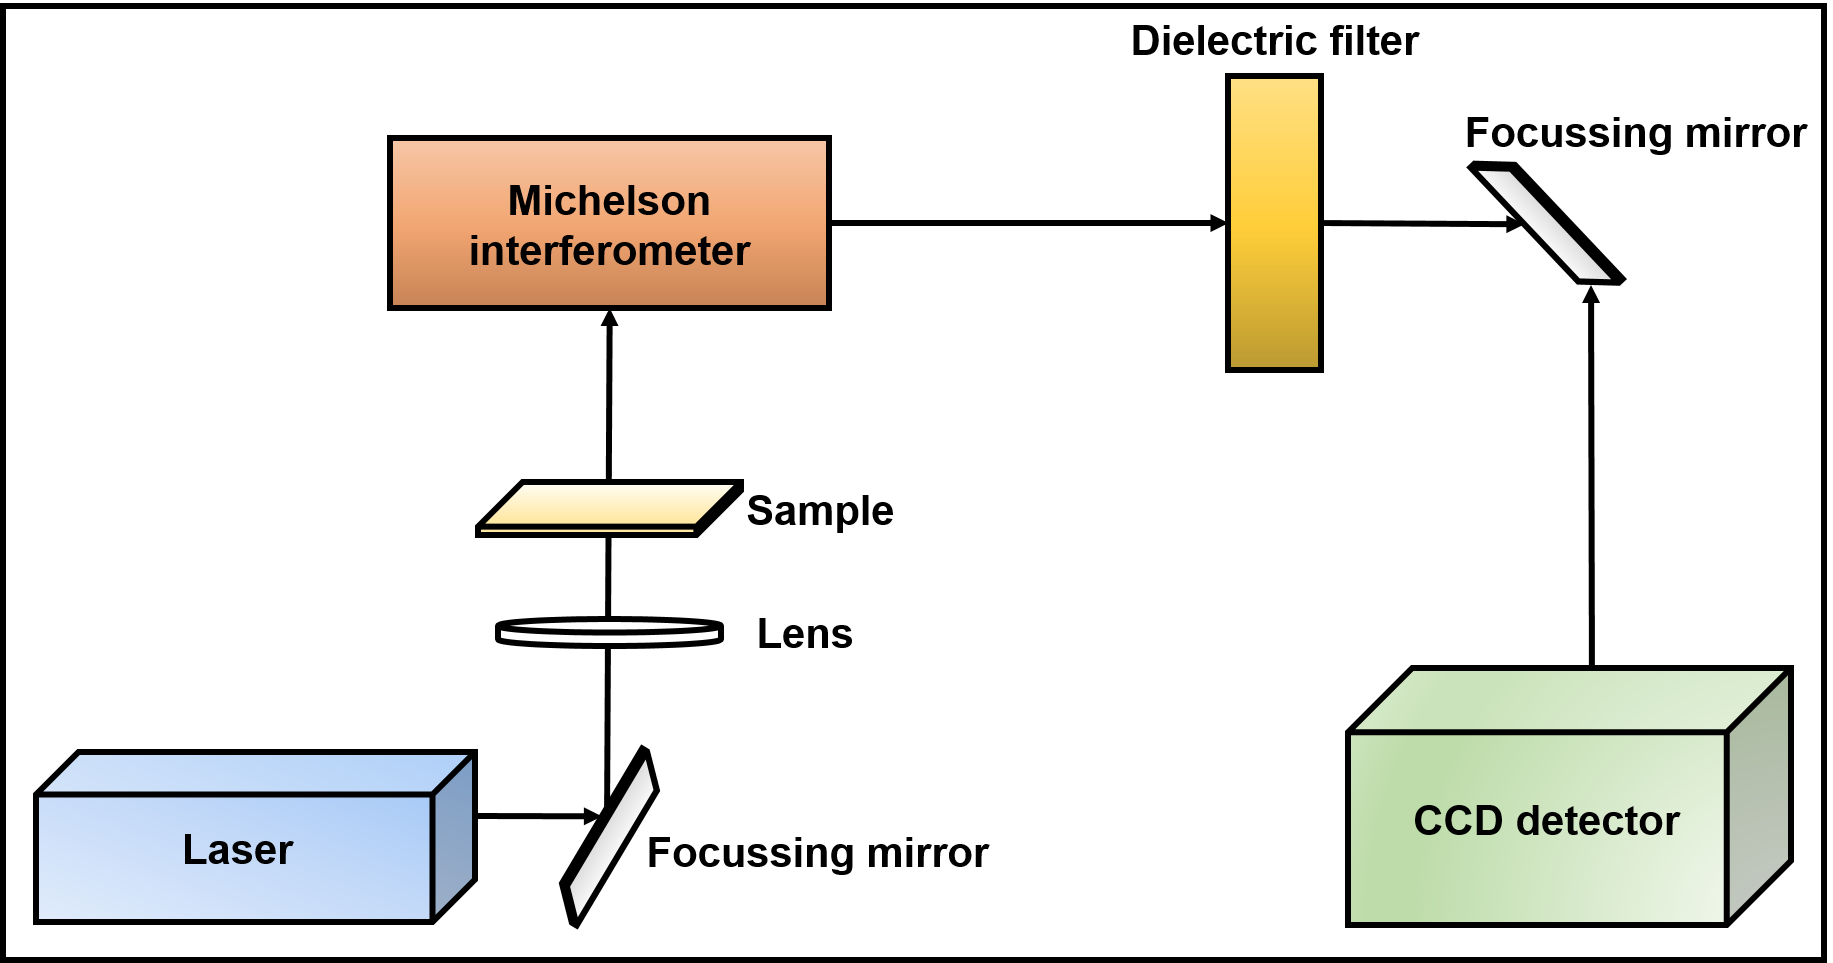
\includegraphics[width=\textwidth]{Figures/Raman}
\caption{Here, the sample is illuminated with a laser beam (blue box). Electromagnetic radiation from the illuminated spot is collected with a lens and sent through a Michelson interferometer (orange box), which produces interference between two beams of light. Elastic scattered radiation at the wavelength corresponding to the laser line is filtered out by a dielectric filter (blocking unwanted wavelengths), while the rest of the collected light is dispersed onto a charged coupled device (CCD)detector, which is a highly sensitive photon detector (green box).}
\label{Figures:Raman}
\end{figure}
This technique uses the inelastic scattering of photons, also known as Raman scattering. A source of monochromatic light, usually from a laser in the visible, near infrared, or near ultraviolet range is used (Figure \ref{Figures:Raman}). The laser light interacts with molecular vibrations, phonons or other excitations in the system, resulting in the energy of the laser photons being shifted up (blue-shift) or down (red-shift). The shift in energy gives information about any changes taking place in the vibrational modes of a material. 

\section{X-ray photoelectron spectroscopy}
\begin{figure}[tbh!]
\centering
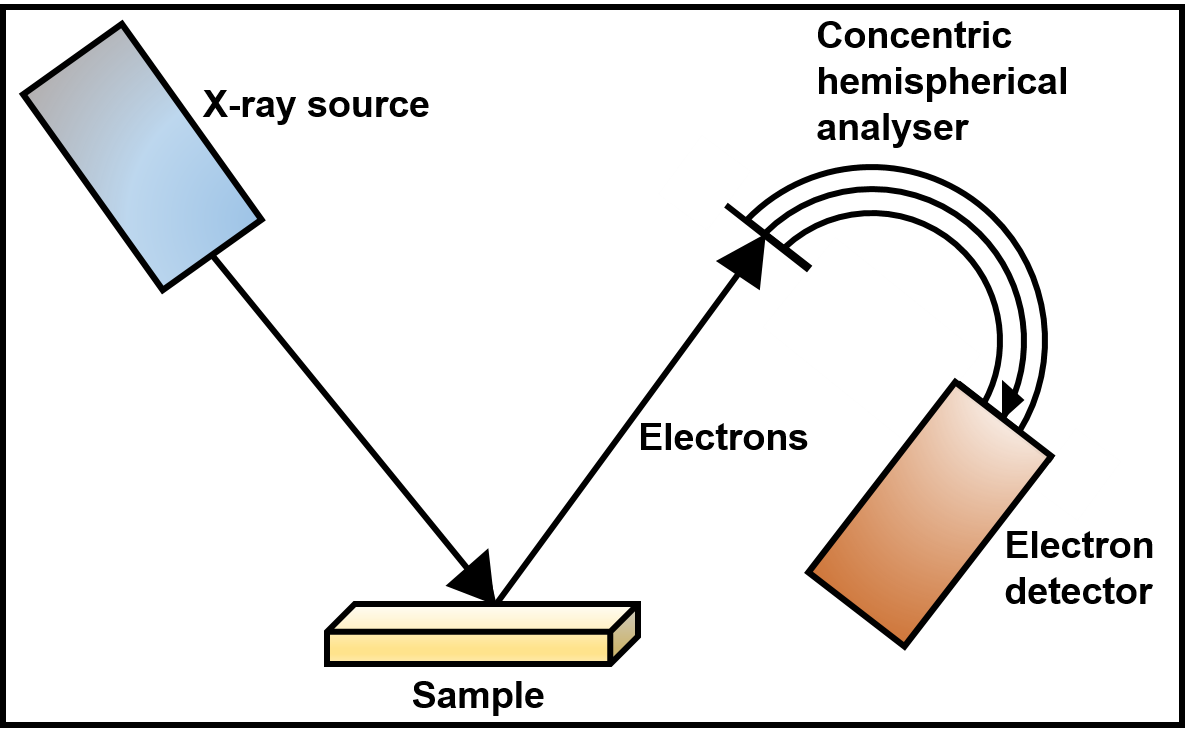
\includegraphics[width=\textwidth]{Figures/XPS}
\caption{}
\label{Figures:XPS}
\end{figure}
To measure elemental composition and oxidation states of various elements, X-ray photoelectron spectroscopy is used. It is a surface-based technique that quantitatively analyses a sample. By irradiating a sample with a beam of X-rays, kinetic energy and number of electrons escaping from the top 10 nm of the sample are measured, in Figure \ref{Figures:XPS}. Since  electron counting detectors in XPS instruments are typically one meter away from the material, a long path length for detection requires low pressures. The instrument requires high vacuum (10$^−^8$ millibar) conditions to count these electrons. The electron emission after irradiation is also called a 'photoelectron effect'. These electrons are separated according to their energies and counted. A normal XPS spectrum is a plot of the number of electrons detected versus the binding energy of the electrons detected. The set of XPS peaks produced at certain binding energies values helps in identifying all the elements, and their chemical environment, that exist in the sample. In practice, XPS detects all elements from lithium and above. It cannot easily detect hydrogen or helium because helium has a very small cross-sectional area for photoemission and hydrogen only has one electron which is used in making bonds with  small photoelectron cross-section. Detection limits for most of the elements are in the parts per thousand range. XPS has been steadily used in batteries to study the different oxidation states of active materials during cell charge/ discharge. One can deduce a battery's mechanism using this tool.
Redox processes taking place inside the each AIB were studied with the help of this technique. For example, in Al/\ce{MoSe2} cells, molybdenum oxidised from \ce{Mo^{+4}} to \ce{Mo^{5+}} when the cells charged. The 2p orbital of Mo had a different binding energy in \ce{MoSe2} in its pristine state but had a different binding energy in \ce{MoO3}. 
\section{Cyclic voltammetry}
\begin{figure}[tbh!]
\centering
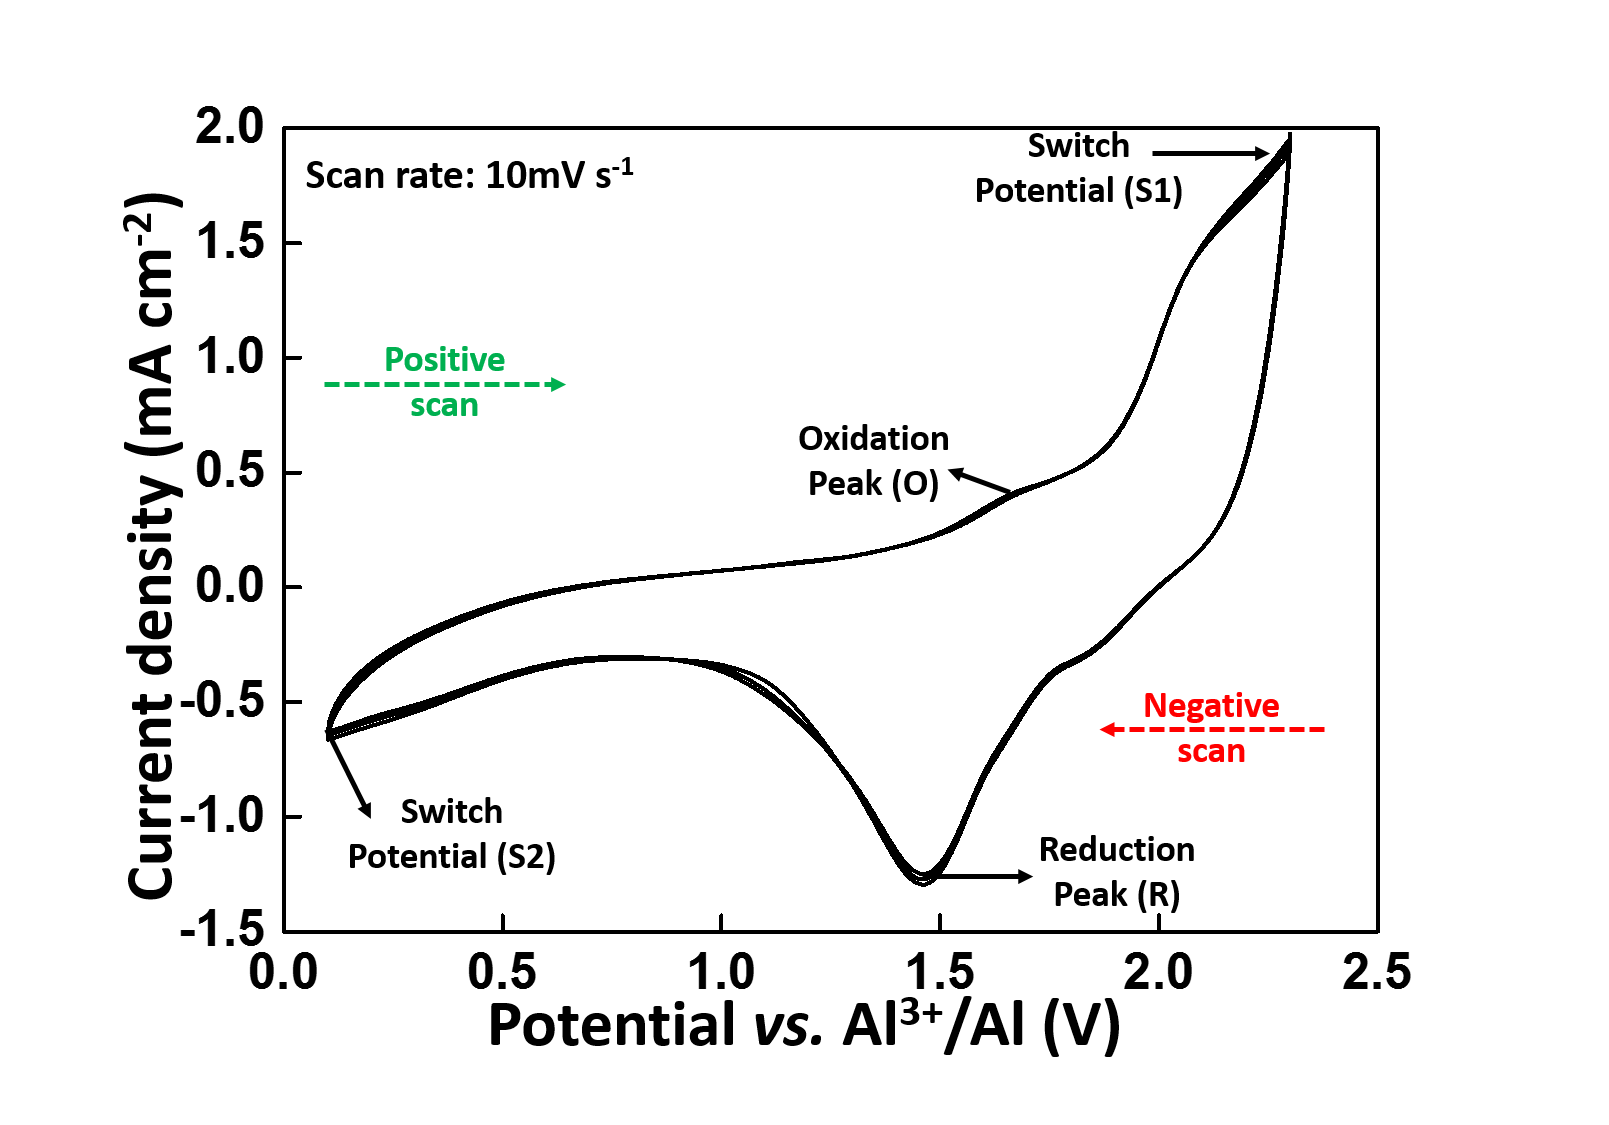
\includegraphics[width=\textwidth]{Figures/CV}
\caption{Cyclic voltammogram of an Al/CFEx cell at a scan rate of 100 mV s$^-^1$ using a two-electrode setup with aluminium acting as both counter and reference electrode. }
\label{Figures:CV}
\end{figure}
Cyclic voltammetry (CV) is a technique which measures the current that develops in an electrochemical cell during oxidation and reduction of an analyte (say M). It is performed by cycling the potential of a working electrode, and measuring the resulting current. The arrow indicates the beginning and sweep direction which can either be forward or reversed, depending on our protocol. In Figure \ref{Figures:CV}, we started a forward sweep with a positive scan (lower potential to higher potential). When the scan reaches a switch potential (voltage is sufficient enough to have caused an oxidation or reduction), S1, it reverses its direction. Potential is then swept negatively (higher potential to lower potential) until it reaches S2 (another switch potential). During forward sweep, M is depleted from the solution as it gets oxidised to \ce{M+}. Further oxidation after scanning higher potentials, leads to growth of a diffusion layer (solution containing M\ce{M+} ions) at the electrode surface throughout the scan. The layer continues to expand until a certain point, recording maximum current density. However, since diffusion layer continues to grow at this stage, flux of M from the bulk solution to electrode surface decreases. Therefore, current starts to decrease and we get an oxidation peak. A reverse scan converts \ce{M+} back to M (reduction) via similar pathway- formation of a diffusion layer containing M and eventually we record a reduction peak. The two peaks are separated due to the diffusion of the analyte to and from the electrode. If the reduction process is chemically and electrochemically reversible, a peak-to-peak separation of 57 mV is observed. Chemical reversibility is used to denote whether the analyte is stable upon reduction and can be easily reoxidised \cite{bard_electrochemical_1980}. When there is a high barrier to electrochemical irreversibility, electron transfer reactions are sluggish and more positive/negative potentials are required to observe oxidation/reduction reactions respectively. Scan rates play a very important role too. If a CV is run on a slower scan rate (0.05 mV s$^-^1$), diffusion layer grows farther from the electrode, which reduces the flux, consequently decreasing the current value. At a faster scan rate lead (1 V s$^-^1$) , a decrease in the size of the diffusion layer is observed and higher currents are observed. Cyclic voltammetry has been a helpful tool in understanding the mechanism of various battery systems i.e. presence of a surface reaction and its reversibility during intercalation/ deintercalation. It not only is valid for single-electron systems, but also for coupled reactions and multi-electron processes.  

\section{Galvanostatic charge/discharge cycles}
Galvanostatic  charge  discharge  is  a  method  to  evaluate  the  electrochemical capacitance of materials under controlled current conditions. This technique is different from cyclic  voltammetry  because the current is controlled and the voltage is  measured. This  method  where current is repeatedly reversed is  also  called  as  'cyclic chronopotentiometry'. It can be used to characterise the electrochemical properties of insertion materials, to estimate their specific capacities and its cycling stability. The total quantity of electricity per mass available from a fully charged cell can be calculated from the charge transferred during discharge in terms of mAh g$^-^1$. Specific discharge capacity is frequently measured at different discharging rates to establish rate capability of a cell. 


